\documentclass{beamer}
\usetheme{Oxygen}
\usepackage{graphicx}
\title{\large  M\'etricas de desempe\~no para Maquinas de Aprendizaje}
\author{Juliana Le\'{o}n, Karen Troiano, Stefano Di Colli}
\begin{document}
\fontfamily{tahoma}
\frame{\titlepage}

\section*{}
\begin{frame}
  \frametitle{\'{I}ndice}
  \tableofcontents[section=1,hidesubsections]
\end{frame}

\AtBeginSection[]
{
  \frame<handout:0>
  {
    \frametitle{\'{I}ndice}
    \tableofcontents[currentsection,hideallsubsections]
	  }
}

\AtBeginSubsection[]
{
  \frame<handout:0>
  {
    \frametitle{\'{I}ndice}
    \tableofcontents[sectionstyle=show/hide,subsectionstyle=show/shaded/hide]
  }
}

\newcommand<>{\highlighton}[1]{%
  \alt#2{\structure{#1}}{{#1}}
}

\newcommand{\icon}[1]{\pgfimage[height=1em]{#1}}

\section{Introducci\'{o}n}

\begin{frame}
  \frametitle{Introducci\'{o}n}
  \begin{block}{M\'etricas para medir desempe\~no}
  \begin{itemize}
  	\item Introduci\'on al problema
    \item Descripci\'on
  \end{itemize}
  \end{block}

\end{frame}

\section{M\'etodos}
\begin{frame}
  \frametitle{M\'etodos Utilizados}
 % \framesubtitle{}

  \begin{block}{M\'etricas}
	\begin{itemize}
	\item Accuracy
	\item Lift
	\item Presion/Recall
	\begin{itemize}
		\item F1
		\item Matthews correlation coefficient
	\end{itemize}
	\item Matriz de Confunsi\'on
	\begin{itemize}
		\item Sensibility
		\item Specificity
	\end{itemize}
	\item ROC - Curva
	\item Coeficiente Silhouette
	\end{itemize}		
	\end{block}
\end{frame}


\begin{frame}
  \frametitle{Accuracy}

  \begin{block}{Descripci\'on}
  \begin{itemize}
  \item Veracidad: Errores Sistem\'aticos
  \item Presi\'on: Errores Random
   
  \end{itemize}
  	
  	\[Accuracy= \dfrac{TP+TN}{TP+FP+FN+TN} \] 
  \end{block}
  \begin{block}{Aplicaciones}
  	Aprendizaje de maquinas donde se cuantan con etiquetas
  	\begin{itemize}
  \item Supervisado
  \item No supervisado
   
  \end{itemize}
  \end{block}
\end{frame}

  	
\begin{frame}
  \frametitle{Lift}

  \begin{block}{Descripci\'on}
  	\begin{itemize}

  	\item Reglas de asociaciones
  	\item Una parte de la data
   
  \end{itemize}
  \end{block}
  \begin{block}{Aplicaciones}

  	\begin{itemize}

  	\item Data Mining
  	\item Marketing
   PONER TABLA
  \end{itemize}
  
  \end{block}
\end{frame}

\begin{frame}
  \frametitle{Presicion/Recall}

  \begin{block}{Descripci\'on}
  	\begin{itemize}

  	\item Presion: Predicci\'on de la clase positiva 
  	\[PPV= \dfrac{TP}{TP+FP} \] 
  	\item Recall: Predicci\'on de la clase negativa
	\[PPV= \dfrac{TN}{TN+FN} \]   
	
  \end{itemize}
  
  \end{block}
 
\end{frame}


\begin{frame}
  \frametitle{F1 score}

  \begin{block}{Descripci\'on}
  	\begin{itemize}
  	\item Presion/Recall
  	\[F1= 2 \dfrac{Presion*Recall}{Presion+Recall} \]   
  	\end{itemize}
  \end{block}
  \begin{block}{Matthews correlation coefficient}
  \begin{itemize}
  	\item Coeficiente de correlaci\'on entre lo observado y lo que se predijo
  	\item Salida : [ -1, 1] 
	\begin{itemize}
	\item -1 : Predici\'on completamente opuesta
	\item 0: No es mejor que random
	\item 1: Predici\'on Perfecta
\end{itemize}	  	
  \end{itemize}
  \end{block}
\end{frame}


\begin{frame}
  \frametitle{Matriz de Confusi\'on}

  \begin{block}{Descripci\'on}
  	Organizacion de los datos para an\'alisis
  	
  	\begin{tabular}{|c|c|c|}
  	\hline 
  	• & Salida Positiva & Salida Negativa \\ 
  	\hline 
  	Real Positiva & TP & FN \\ 
  	\hline 
  	Real Negativa & FP & TN \\ 
  	\hline 
  	\end{tabular} 
  \end{block}
  \begin{block}{M\'etricas obtenidas}
  \begin{itemize}
  	\item Sensitivity: \[TPR=  \dfrac{TP}{TP+FN} \]   
  	\item Specificity: \[TNR=  \dfrac{TN}{FP+TN} \]   
	\item No datos desbalanceados
    \end{itemize}
  
  \end{block}
\end{frame}


\begin{frame}
  \frametitle{ROC}

  \begin{block}{Descripci\'on}
  	\begin{itemize}
  	\item Graficar Sensitivity x Specificity
  	\item Datos desbalanceados
  	\item Medicina y Biolog\'ia
  	\end{itemize}
  \end{block}

  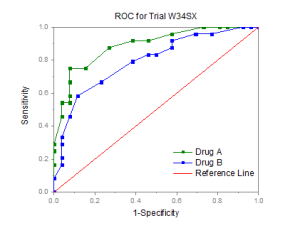
\includegraphics[scale=0.7]{roc.png} 
\end{frame}

\begin{frame}
  \frametitle{Coeficiente de Silhouette}
  \begin{block}{Descripci\'on}
  \begin{itemize}
  \item Es un coeficiente usado para validar Clusters
  	\item Por cada valor exite un coeficiente Silhouette que representa la clase 
  \end{itemize}
  	
  \end{block}
\end{frame}


\section{Resumen}
\begin{frame}
\frametitle{Resumen}
\begin{block}{}
	\begin{itemize}
	 \item Variedad de metricas
	 \item Adaptivilidad
	 \item Accuracity no es suficiente
	 \item ROC y Matriz de confusion 
	 \item Sin los datos etiquetados en un problema mas completo
	\end{itemize}  
\end{block}

\end{frame}

\begin{frame}

\LARGE{PREGUNTAS}
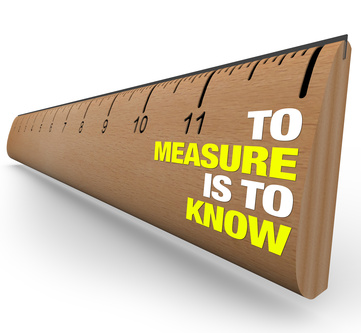
\includegraphics[scale=0.5]{measure.jpg} 
\end{frame}
\end{document}